% =====================================================================
% Chapter 4 -- Data Description
%
% Every paragraph is a CLAUDE-DRAFT (2026-10-19) to be rewritten by the author.
% Sources of the facts: thesis_notes.md (dataset papers, official SKM-TEA
% documentation and annotation files, code, HPC statistics run of 2026-10-19),
% paper_notes/voxtell.md, results/data_stats/.
% Tables and figures are generated by scripts/plot_data.py; do not edit them.
% =====================================================================

\chapter{Data Description}
\label{chap:data}

% CLAUDE-DRAFT
This chapter describes the two public datasets used in this thesis.
SKM-TEA~\cite{desai2021skmtea} provides the knee \gls{mri} volumes from which the six continual-learning tasks are built, and AeroPath~\cite{støverud2023aeropathairwaysegmentationbenchmark} provides the chest \gls{ct} volumes of the control task, a held-out task that is never trained on.
\cref{tab:ch4_datasets} summarises both datasets.
The chapter then describes how the volumes are split, how the few-shot training subsets are drawn, how the data are preprocessed, and which properties of the data limit the conclusions that can be drawn from them.

\begin{table}[tb]
\centering
\caption{Datasets used in this thesis. Values computed from the data and the official SKM-TEA annotation files (version 1.0.0), except imaging, source and access, which are taken from the dataset publications~\cite{desai2021skmtea, støverud2023aeropathairwaysegmentationbenchmark}.}
\label{tab:ch4_datasets}
% Generated by scripts/plot_data.py from results/data_stats and the dataset papers. Do not edit.
\small\setlength{\tabcolsep}{4pt}
\begin{tabular}{@{}l>{\raggedright\arraybackslash}p{0.34\linewidth}>{\raggedright\arraybackslash}p{0.34\linewidth}@{}}
\toprule
 & SKM-TEA & AeroPath \\
\midrule
Role in this thesis & six continual-learning tasks & control task \\
Imaging & MRI, 3D qDESS, echo 1 & CT angiography \\
Source & Stanford Healthcare & St. Olavs hospital \\
Volumes used (patients) & 155 (155) & 27 (27) \\
With pathology label$^{a}$ & 130 of 155 & -- \\
Split (train/val/test) & 108/23/24 & 19/4/4 \\
Volume size (voxels) & 512 $\times$ 512 $\times$ 144--168 & 487--512 $\times$ 407--512 $\times$ 241--843 \\
Voxel size (mm) & 0.3125 $\times$ 0.3125 $\times$ 0.8$^{b}$ & 0.56--0.82 $\times$ 0.56--0.82 $\times$ 0.50--1.25 \\
Structures used & 6 (Table~\ref{tab:ch4_structures}) & lung \\
Access & \url{github.com/StanfordMIMI/skm-tea} & \url{github.com/raidionics/AeroPath} \\
\bottomrule
\end{tabular}
\par\smallskip{\footnotesize\raggedright $^{a}$ At least one pathology bounding box in the official SKM-TEA annotation files (cartilage lesion, effusion, meniscal tear, ligament tear).\par $^{b}$ From the official annotation files; the NIfTI files used in this thesis store an identity affine (1\,mm).\par}

\end{table}

% ---------------------------------------------------------------------
\section{SKM-TEA}
\label{sec:data-skmtea}

\subsection{Acquisition and Annotation}
\label{subsec:data-skmtea-acquisition}

% CLAUDE-DRAFT
The Stanford Knee MRI with Multi-Task Evaluation (SKM-TEA) dataset contains knee \gls{mri} scans of 155 patients acquired at Stanford Healthcare~\cite{desai2021skmtea}.
All scans were acquired with the 3D \gls{qdess} sequence on one of two 3\,T GE MR750 scanners, with patient consent and approval of the Stanford University Institutional Review Board~\cite{desai2021skmtea}.
\gls{qdess} acquires two inherently registered 3D echoes with different contrasts~\cite{desai2021skmtea}.
The shared acquisition parameters are a matrix of $416 \times 512$ (readout $\times$ phase encoding), an in-plane resolution of $0.38 \times 0.31$\,mm$^2$, echo times of 5.7\,ms and 30.1\,ms, a repetition time of 17.9\,ms, a flip angle of 20$^\circ$ and 80 to 88 slices depending on knee size~\cite[Table~5, App.~A.1]{desai2021skmtea}.

% CLAUDE-DRAFT
SKM-TEA is distributed in two benchmark tracks, one based on raw k-space data and one based on the scanner-generated \gls{dicom} images~\cite{desai2021skmtea}.
We use the \gls{dicom} track, which stores the images and segmentations of each scan in one \gls{hdf5} file\footnote{\url{https://github.com/StanfordMIMI/skm-tea/blob/main/DATASET.md}, accessed 19 October 2026.}.
Of the two echoes, we use only the first, as the dataset authors do in the segmentation part of their tutorial~\cite{skmtea_tutorial}.
According to the official annotation files, all 155 volumes have a voxel size of $0.3125 \times 0.3125 \times 0.8$\,mm and a matrix of $512 \times 512$ voxels with 160 slices, except four volumes with 144, 152, 156 and 168 slices.

% CLAUDE-DRAFT
Six tissues were segmented manually on all \gls{dicom} images: patellar cartilage, femoral cartilage, medial and lateral tibial cartilage, and medial and lateral meniscus~\cite{desai2021skmtea}.
The segmentations were drawn slice by slice in the sagittal plane by two researchers with three to four years of experience in knee \gls{mri} interpretation, supervised by two board-certified musculoskeletal radiologists, and corrected for volumetric consistency in the axial and coronal planes~\cite[App.~A.4]{desai2021skmtea}.
Each scan was labelled by a single annotator~\cite[App.~A.4]{desai2021skmtea}.
The dataset also provides bounding boxes for sixteen pathology categories~\cite{desai2021skmtea}.
According to the annotation files, 130 of the 155 scans contain at least one pathology: 99 a cartilage lesion, 88 an effusion, 68 a meniscal tear and 36 a ligament tear.
These bounding boxes are not used for training or evaluation in this thesis.

% CLAUDE-DRAFT
SKM-TEA is distributed under the terms of the Stanford University School of Medicine and of the Lower Extremity Radiographs dataset~\cite[App.~A.5]{desai2021skmtea}, and we signed the Stanford AIMI research-use agreement before downloading the data.

\subsection{Continual-Learning Tasks}
\label{subsec:data-skmtea-tasks}

% CLAUDE-DRAFT
Each of the six segmented structures defines one task, with a fixed text prompt that names the structure (\cref{tab:ch4_structures}).
The same text prompt is used for training and evaluation, and its wording is not varied.
Since all six structures are labelled in every volume, the six tasks share the same 155 volumes and differ only in the target structure.
The order in which the tasks are trained is part of the experimental setup and is given in the Experiment and Results chapter.\todo{ref: task order section}

\begin{table}[tb]
\centering
\caption{Structures of the six continual-learning tasks and of the control task, with the text prompt, the label value in the converted label maps (\cref{sec:data-preprocessing}) and the structure volume over all volumes of the dataset. SKM-TEA volumes are computed from the voxel counts and the voxel size of the official annotation files; AeroPath volumes from the voxel size stored in each file.}
\label{tab:ch4_structures}
% Generated by scripts/plot_data.py from results/data_stats. Do not edit.
\small\setlength{\tabcolsep}{4pt}
\begin{tabular}{lllr}
\toprule
Task & Text prompt & Label & Volume (cm$^3$), median [IQR] \\
\midrule
Lateral tibial cartilage & ``lateral tibial cartilage'' & 4 & 2.32 [1.82, 2.96] \\
Medial tibial cartilage & ``medial tibial cartilage'' & 3 & 2.13 [1.75, 2.56] \\
Femoral cartilage & ``femoral cartilage'' & 2 & 10.99 [8.73, 13.50] \\
Patellar cartilage & ``patellar cartilage'' & 1 & 3.14 [2.35, 3.77] \\
Medial meniscus & ``medial meniscus'' & 5 & 2.20 [1.81, 2.69] \\
Lateral meniscus & ``lateral meniscus'' & 6 & 1.90 [1.50, 2.37] \\
\midrule
Control task (AeroPath) & ``lung'' & -- & 4\,858 [3\,732, 6\,231] \\
\bottomrule
\end{tabular}

\end{table}

% CLAUDE-DRAFT
The structures differ in size (\cref{fig:ch4_structure_sizes}).
Femoral cartilage is the largest structure, with a median volume of 10.99\,cm$^3$, while the medians of the other five structures lie between 1.90\,cm$^3$ (lateral meniscus) and 3.14\,cm$^3$ (patellar cartilage).
The six structures lie next to each other in the knee joint, as the example in \cref{fig:ch4_examples} shows.

\begin{figure}[tb]
\centering
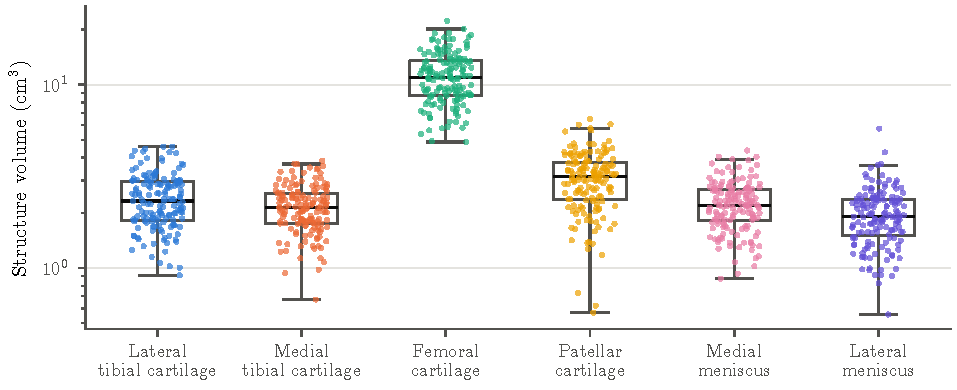
\includegraphics[width=\linewidth]{figures/ch4_structure_sizes.pdf}
\caption{Volume of each SKM-TEA structure over all 155 volumes (logarithmic axis). Boxes show the median and the interquartile range, whiskers extend to 1.5 times the interquartile range, and each point is one volume.}
\label{fig:ch4_structure_sizes}
\end{figure}

\begin{figure}[tb]
\centering
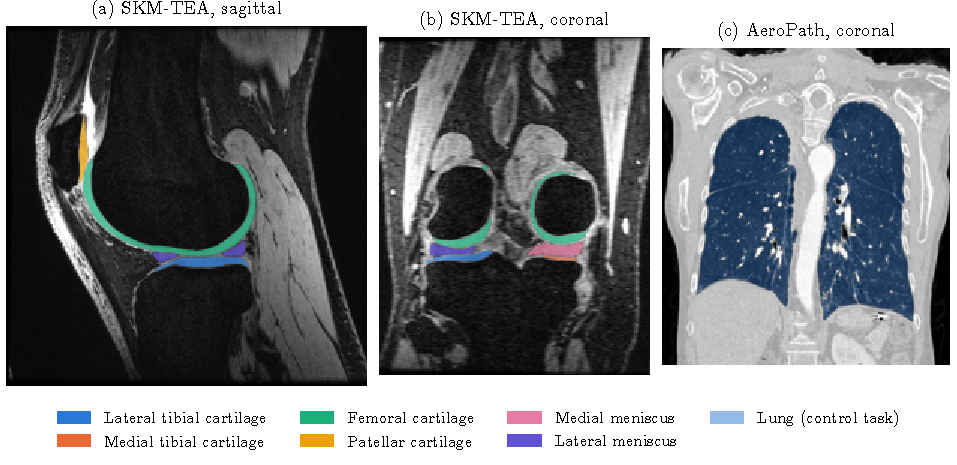
\includegraphics[width=\linewidth]{figures/ch4_examples.pdf}
\caption{Example volumes with their labels. (a)~Sagittal slice of SKM-TEA volume MTR\_005 through the lateral compartment, showing patellar, femoral and lateral tibial cartilage and the lateral meniscus. (b)~Coronal slice of the same volume through the tibial plateau, showing femoral cartilage, both tibial cartilages and both menisci. (c)~Coronal slice of AeroPath volume~1 with the lung label of the control task. Both example volumes belong to the test split.}
\label{fig:ch4_examples}
\end{figure}

% CLAUDE-DRAFT
We chose SKM-TEA because VoxTell performs poorly on it.
In the zero-shot evaluation of its authors, VoxTell reaches a mean Dice score of 10.72\,\% over the six SKM-TEA structures, with 46.45\,\% for femoral cartilage and at most 14.78\,\% for the other structures~\cite[Table~9]{rokuss2025voxtellfreetextpromptableuniversal}.
The authors attribute this to the knee being sparsely represented in the training data, and they name few-shot adaptation with minimal labelled examples as future work~\cite[p.~8]{rokuss2025voxtellfreetextpromptableuniversal}.
The knee is not entirely absent from VoxTell's training data, however: its label vocabulary contains femoral, patellar, and medial and lateral tibial cartilage from two knee \gls{mri} datasets, but no meniscus~\cite[Tables~4, 5 and~10]{rokuss2025voxtellfreetextpromptableuniversal}.
According to this vocabulary, SKM-TEA therefore combines structures that VoxTell has rarely seen with structures it has never seen.

% ---------------------------------------------------------------------
\section{AeroPath}
\label{sec:data-aeropath}

% CLAUDE-DRAFT
AeroPath contains 27 contrast-enhanced chest \gls{ct} scans (\gls{cta}), acquired with a thorax lung protocol at St.\ Olavs hospital in Trondheim, Norway~\cite{støverud2023aeropathairwaysegmentationbenchmark}.
The 27 patients, nine of them women, were aged 52 to 84 years (median 70) and were all undergoing diagnostic tests for lung cancer, with pathologies including malignant tumours, sarcoidosis and emphysema~\cite{støverud2023aeropathairwaysegmentationbenchmark}.
Data collection was approved by the Norwegian regional ethics committee (REK Sør-Øst~A, reference 2010/3385a), and written informed consent was obtained from the patients~\cite{støverud2023aeropathairwaysegmentationbenchmark}.
The dataset is distributed under the Creative Commons Attribution 4.0 licence\footnote{Zenodo record \url{https://zenodo.org/records/10069289}, DOI 10.5281/zenodo.10069289, accessed 19 October 2026.}.

% CLAUDE-DRAFT
In the files used here, the volumes have 487 to 512 by 407 to 512 voxels in-plane and 241 to 843 slices, with an in-plane voxel size of 0.56 to 0.82\,mm and a slice spacing of 0.50 to 1.25\,mm.
These ranges are wider than those stated in the dataset publication~\cite{støverud2023aeropathairwaysegmentationbenchmark}; we report the values of the files.
Each volume comes with an airway label and a lung label.
The publication describes how the airway labels were created, by region growing or grow-cut, an airway segmentation network and manual refinement verified by a pulmonologist~\cite{støverud2023aeropathairwaysegmentationbenchmark}.
How the lung labels were created is documented neither in the publication nor in the dataset repository or the Zenodo record.
We use only the lung label, with the text prompt ``lung''.

% CLAUDE-DRAFT
AeroPath serves as the control task.
It is never trained on, except by the strategy with replay, whose replay memory includes AeroPath training volumes.\todo{ref: Method, replay}
It measures how much of the pretrained model's ability on a structure outside the task sequence is lost during continual adaptation.
We chose it because the pretrained model segments it well and because it is public.
AeroPath is not part of VoxTell's training data: its authors use it as a held-out test set for a known concept, on which VoxTell reaches a lung Dice score of 96.99\,\%~\cite[Table~7]{rokuss2025voxtellfreetextpromptableuniversal}.
The concept itself is well represented in VoxTell's training data, where ``lung'' is among the most frequent labels~\cite[Table~10]{rokuss2025voxtellfreetextpromptableuniversal}.
How the loss of this ability is quantified is defined in the Method chapter.\todo{ref: control-task drop}

% ---------------------------------------------------------------------
\section{Data Splits and Few-Shot Subsets}
\label{sec:data-splits}

% CLAUDE-DRAFT
We split each dataset once, at random, into 70\,\% training, 15\,\% validation and 15\,\% test volumes.
The volumes are shuffled with a fixed random seed (42), the first 70\,\% of the shuffled list form the training split and the next 15\,\% the validation split, and the remaining volumes form the test split.
This gives 108 training, 23 validation and 24 test volumes for SKM-TEA and 19, 4 and 4 volumes for AeroPath.
Because the six tasks share the same volumes, every task uses the same split, and every experiment in this thesis uses the same split.
Each SKM-TEA patient contributes exactly one scan, so no patient appears in more than one split.
The validation volumes are used to select the checkpoint of each task; all reported results are computed on the test volumes.\todo{ref: Method, checkpoint selection}

% CLAUDE-DRAFT
SKM-TEA also defines an official split of 86 training, 33 validation and 36 test scans, in which the test scans are those of the 36 patients who received additional arthroscopic surgery~\cite{desai2021skmtea}.
We do not use this split, for two reasons.
First, the aim of this thesis is to compare continual-learning strategies with each other, not to compare results with published SKM-TEA benchmarks, which is the purpose of the official split; the comparison only requires that all strategies use the same split.
Second, the official test set consists of a selected group of patients, so a model trained on the official training split is tested under a shift between training and test data.
A random split keeps training and test volumes from the same distribution, so that differences in adaptation and forgetting are not mixed with the effect of such a shift.
\cref{tab:ch4_splits} shows how the official splits are distributed over our splits: 7 of our 24 test volumes belong to the official test set.
The results of this thesis are therefore not comparable with results reported on the official SKM-TEA test set.

\begin{table}[tb]
\centering
\caption{Number of SKM-TEA volumes in each split of this thesis (rows) and of the official SKM-TEA split~\cite{desai2021skmtea} (columns).}
\label{tab:ch4_splits}
% Generated by scripts/plot_data.py from results/data_stats. Do not edit.
\small\setlength{\tabcolsep}{6pt}
\begin{tabular}{lrrrr}
\toprule
 & \multicolumn{3}{c}{Official SKM-TEA split} & \\
\cmidrule(lr){2-4}
This thesis & Train & Val. & Test$^{a}$ & Total \\
\midrule
Training & 63 & 22 & 23 & 108 \\
Validation & 10 & 7 & 6 & 23 \\
Test & 13 & 4 & 7 & 24 \\
\midrule
Total & 86 & 33 & 36 & 155 \\
\bottomrule
\end{tabular}
\par\smallskip{\footnotesize $^{a}$ Patients with additional arthroscopic surgery.\par}

\end{table}

% CLAUDE-DRAFT
For the few-shot experiments, the training split of each task is reduced to its first $k$ volumes, with $k \in \{5, 10, 20\}$ labelled training volumes per task, in the order of the shuffled list.
The subsets are therefore nested, the 5 volumes being part of the 10 and the 10 part of the 20, and the same volumes are used for all six tasks.
For each $k$, one subset is drawn, so the results do not show how they vary with the choice of training volumes.
The full-data setting uses all 108 training volumes, and the validation and test volumes are the same in all settings.

% CLAUDE-DRAFT
Of AeroPath, only the 4 test volumes are used for evaluation.
The 19 training volumes are used only by the replay strategy, and the 4 validation volumes are not used.

% ---------------------------------------------------------------------
\section{Preprocessing}
\label{sec:data-preprocessing}

% CLAUDE-DRAFT
We convert each SKM-TEA \gls{hdf5} file into two \gls{nifti} files, one for the first echo and one for the labels.
The segmentation is stored as six binary channels, one per tissue; we convert it into a single label map in which each labelled voxel takes the index of its channel plus one and unlabelled voxels take the value zero.
Following the channel order of the official documentation, the label values are 1 for patellar cartilage, 2 for femoral cartilage, 3 for medial tibial cartilage, 4 for lateral tibial cartilage, 5 for medial meniscus and 6 for lateral meniscus.
For each task, the binary target mask consists of the voxels with the task's label value.
The \gls{nifti} files are written with an identity affine, so they store neither the voxel size nor the orientation of the scan.
Images and labels come from the same voxel grid and therefore stay aligned, which we checked visually in ITK-SNAP.\todo{cite: ITK-SNAP}
The AeroPath volumes and labels are used in their original \gls{nifti} format.

% CLAUDE-DRAFT
When a volume is loaded, it is reoriented according to its affine, which leaves the SKM-TEA volumes unchanged, and cropped to the bounding box of its non-zero voxels.
Its intensities are then normalised to zero mean and unit standard deviation over the cropped volume, using the z-score normalisation of nnU-Net~\cite{isensee2018nnunetselfadaptingframeworkunetbased}.
The same normalisation is applied to the \gls{mri} and the \gls{ct} volumes.
The volumes are not resampled.
The SKM-TEA volumes are therefore processed on their voxel grid as if the voxels were 1\,mm cubes, while the AeroPath volumes keep their physical voxel size.
How patches are sampled during training and how predictions are assembled during evaluation is described in the Method chapter.\todo{ref: Method, patch sampling and sliding-window inference}

% ---------------------------------------------------------------------
\section{Data Quality and Limitations}
\label{sec:data-limitations}

% CLAUDE-DRAFT
Several properties of the data limit the conclusions of this thesis.
Because of the identity affine, the SKM-TEA volumes reach the model at a different scale than their physical size: a voxel of $0.3125 \times 0.3125 \times 0.8$\,mm is treated as a 1\,mm cube, which enlarges the in-plane extent by a factor of 3.2 and the slice direction by a factor of 1.25.
The AeroPath volumes, in contrast, keep their physical voxel size, so the two datasets are processed at different scales.
Whether either scale matches the data on which VoxTell was pretrained cannot be checked from its publication, which does not state the voxel size used for training~\cite{rokuss2025voxtellfreetextpromptableuniversal}.\todo{defense: SKM-TEA scale and missing resampling may contribute to the low performance of the pretrained model on SKM-TEA; check the official VoxTell preprocessing}
The identity affine also removes the orientation: 18 of the 155 SKM-TEA scans are stored with the left--right axis reversed relative to the other 137, and the model receives them without this information.

% CLAUDE-DRAFT
The model sees only the first \gls{qdess} echo, although the annotators used both echoes to separate neighbouring cartilage and meniscus voxels~\cite[App.~A.4]{desai2021skmtea}.
Each SKM-TEA scan was labelled by one annotator, so the data contain no information on the agreement between annotators.
For AeroPath, the origin of the lung labels is not documented, so it is unknown whether they are manual or automatic references.
The control task is evaluated on only four test volumes, which makes its results less certain than those of the SKM-TEA tasks with 24 test volumes.
The \gls{ct} volumes are normalised per volume like the \gls{mri} volumes; whether this matches the normalisation used to pretrain VoxTell is not stated in its publication.\todo{defense: check VoxTell's CT intensity normalisation}
Finally, every result depends on one random split of each dataset and on one subset per number of training volumes.
